GNSS (Global Navigation Satellite System) er samlebetegnelsen for alle satellittbaserte posisjoneringssystemer som brukes for finne posisjon på 
jordens overflate. Amerikanske NAVSTAR, som var det første operative systemet. Ble fullt utbygd på 1990-tallet og 
var i utgangspunktet tiltenkt militær bruk. Under utviklingen av systemet ble det i tillegg tilgjengelig for det sivile. 
Etter hvert har andre systemer kommet til, slik som GLONASS (Russisk), Galileo (Europeisk) og BeiDou (Kinesisk). \parencite{ForsellGNSS}

\subsubsection{Funksjon}

Felles for alle disse systemene er at avstanden fra en GNSS-mottaker til satellittene brukes til å beregne mottakerens posisjon 
ved hjelp av triangulering. For å triangulere en 2D-posisjon behøves kommunikasjon med tre satellitter, og fire for å kunne definere 
høyden til mottakeren. Jo flere satellittsignaler som benyttes i trianguleringen, jo bedre posisjonsnøyaktighet er det mulig å oppnå. 
\parencite{NorskRomsenter}

Systemene fungerer ved at hver satellitt har et atomur som går svært nøyaktig med neglisjerbare avvik. 
En satellittmottaker har ikke tilsvarende nøyaktig klokke, men mottar jevnlig synkroniseringsdata fra satellittene. 
I tillegg går satellittene i kjente baner, slik at mottakeren på bakken til enhver tid vet hvor satellittene befinner seg. 
Ved å sammenligne tidspunktet signalet ble sendt med tidspunktet signalet ble mottatt, 
kan systemet beregne avstanden til mottakere ved hjelp av «time of flight»-beregning vist i figur \ref{fig:code-positioning}. 
Denne beregningen kan gjøres på flere måter, som igjen vil kunne gi forskjellig nøyaktighet i posisjoneringen. \parencite{ForsellGNSS} 

\begin{figure}[htp]
    \centering
    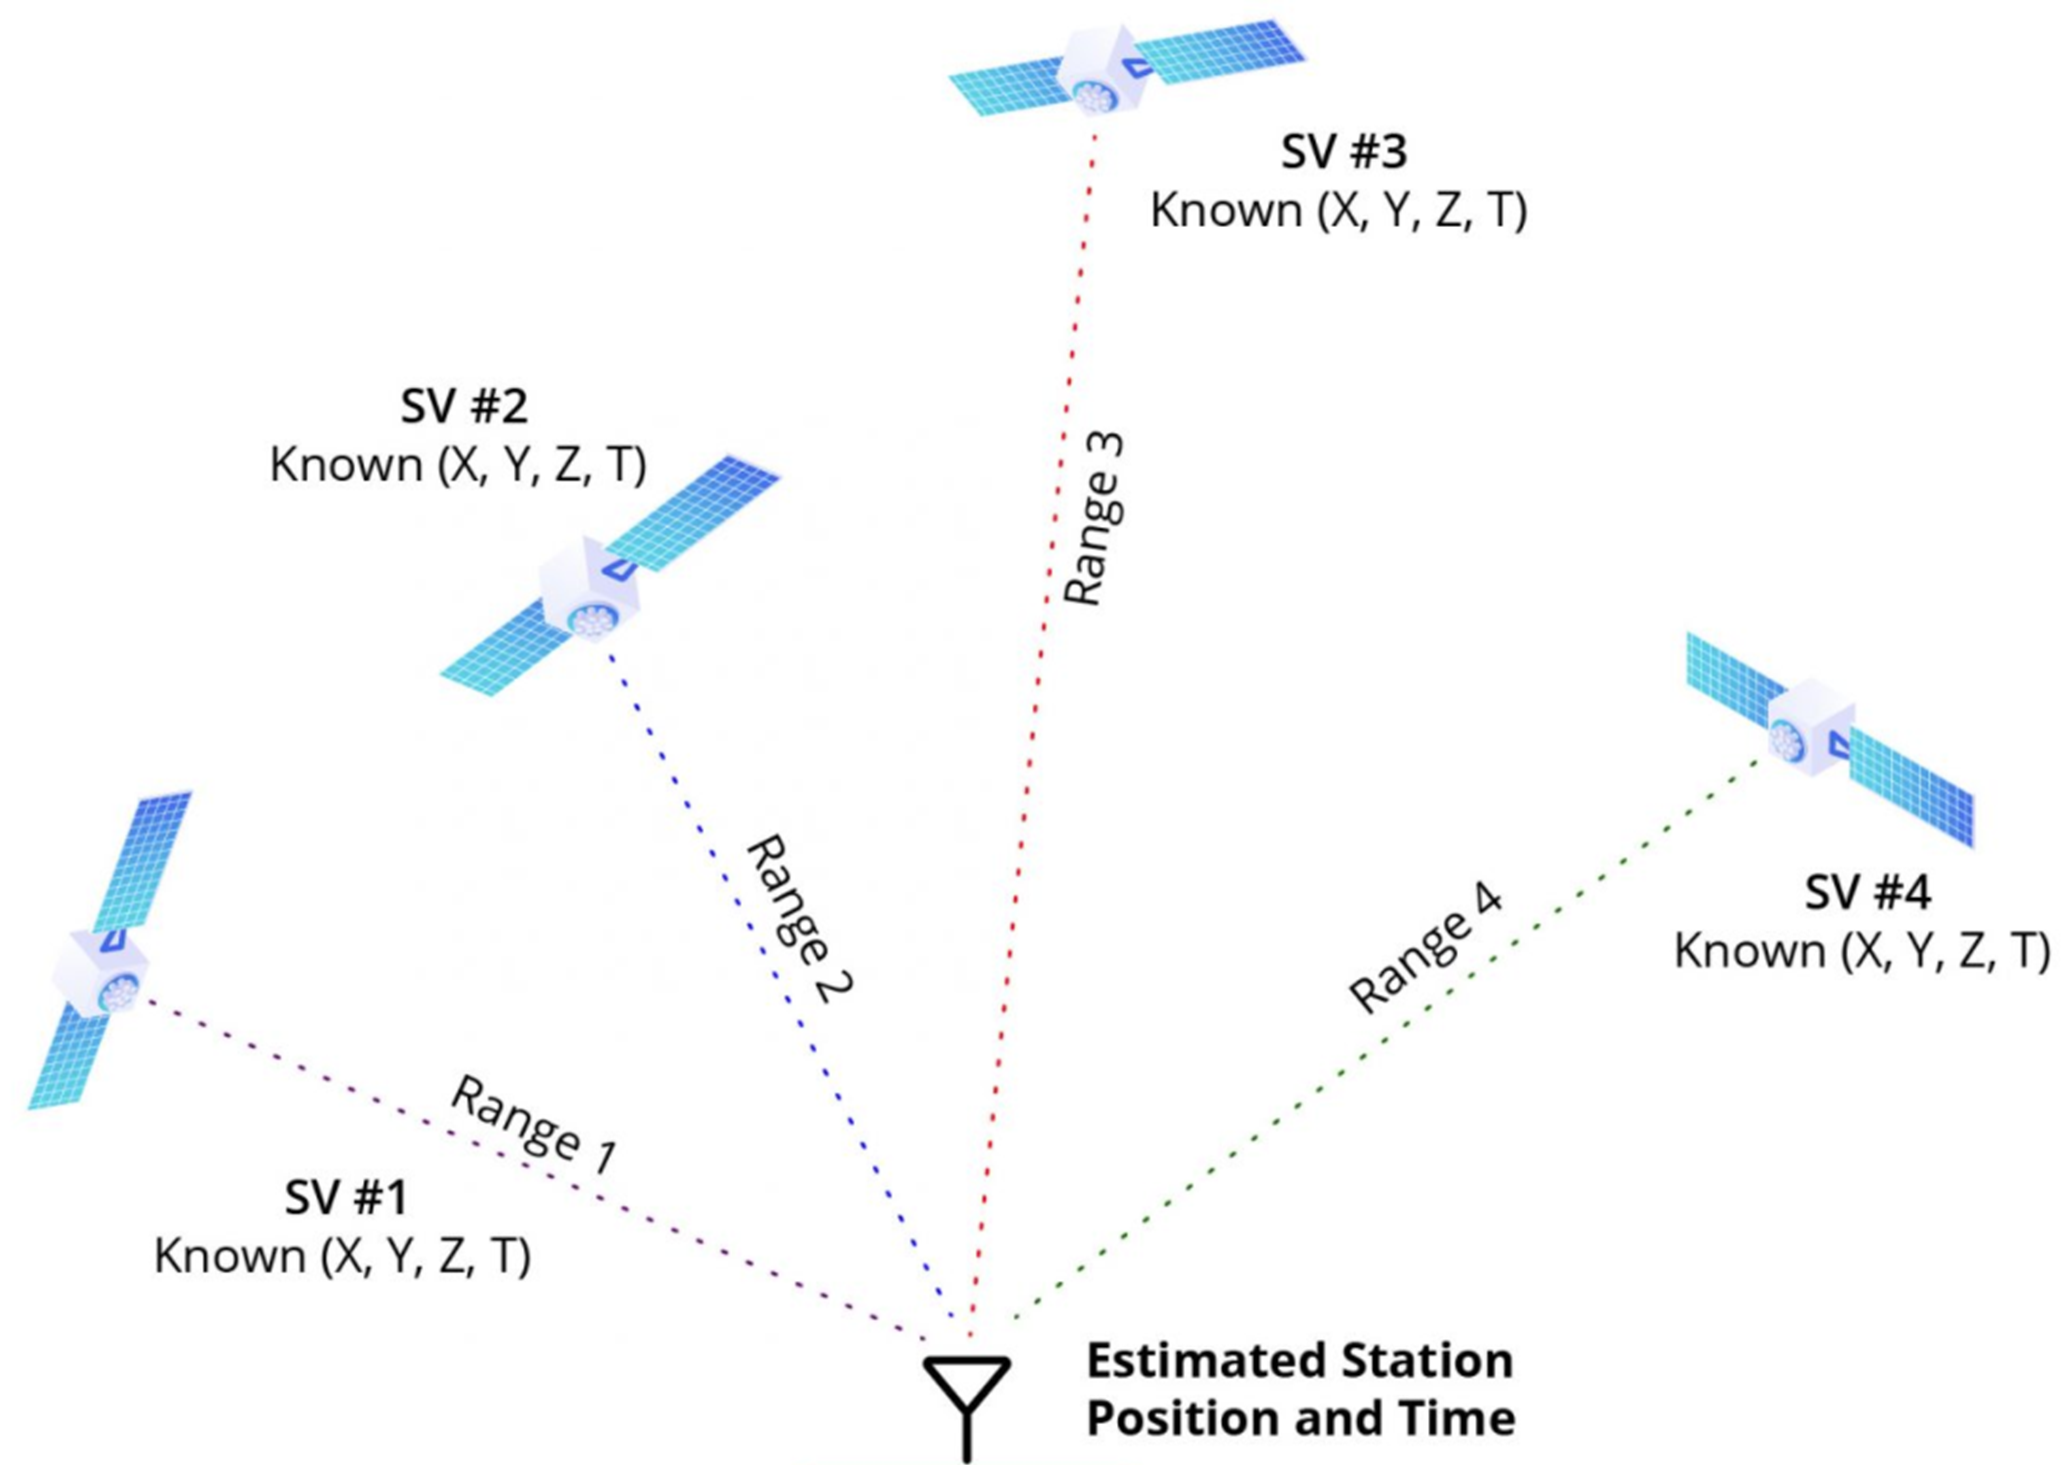
\includegraphics[width=1\columnwidth]{figures/code-positioning}
    \caption{Code-positioning. \parencite{Tallysman}}
    \label{fig:code-positioning}
\end{figure}

Teoretisk sett kan nøyaktigheten i avstandsbestemmelsen fra en GNSS-mottaker til en GNSS-satellitt være omkring 1 meter for den 
enkleste formen for avstandsberegning (beregnet ut ifra det amerikanske systemet). Videre kan mer avanserte metoder som 
fasemåling gjøre at den teoretiske nøyaktigheten kommer ned mot millimeternøyaktighet da bølgelengden til bærefrekvensen L1 er på 19 cm. 
Fasene er periodiske og derfor kan ikke fasemåling brukes alene, da dette vil gi mange mulige avstander til satellittene. 
En tredje metode er differensiell måling, hvor en basestasjon ved et fastpunkt med kjent posisjon måler avvik mellom 
målt posisjon og faktisk posisjon. Dette avviket sendes så til en GNSS-sensor i nærheten som benytter avviket til å beregne 
en svært nøyaktig posisjon. Jo nærmere GNSS-sensoren er fastpunktet, jo mer korrekt er avviksdataen og dermed blir den målte 
posisjonen mer korrekt. \parencite{ForsellGNSS}

\subsubsection{Nøyaktighet}
I bruk kan man ikke forvente å oppnå den teoretiske nøyaktigheten, da det er svært mange feilkilder som påvirker posisjoneringen. 
For å estimere hvor nøyaktig systemene faktisk er så benytter man begrepet «User Range Error» (URE) fra satellitten. 
I 1990 var URE omkring 4.6 meter, og i 2019 var gjennomsnittlig URE nede på cirka 0,5 meter. \parencite{ForsellGNSS}

\subsubsection{Feilkilder}

\begin{figure}[htp]
    \centering
    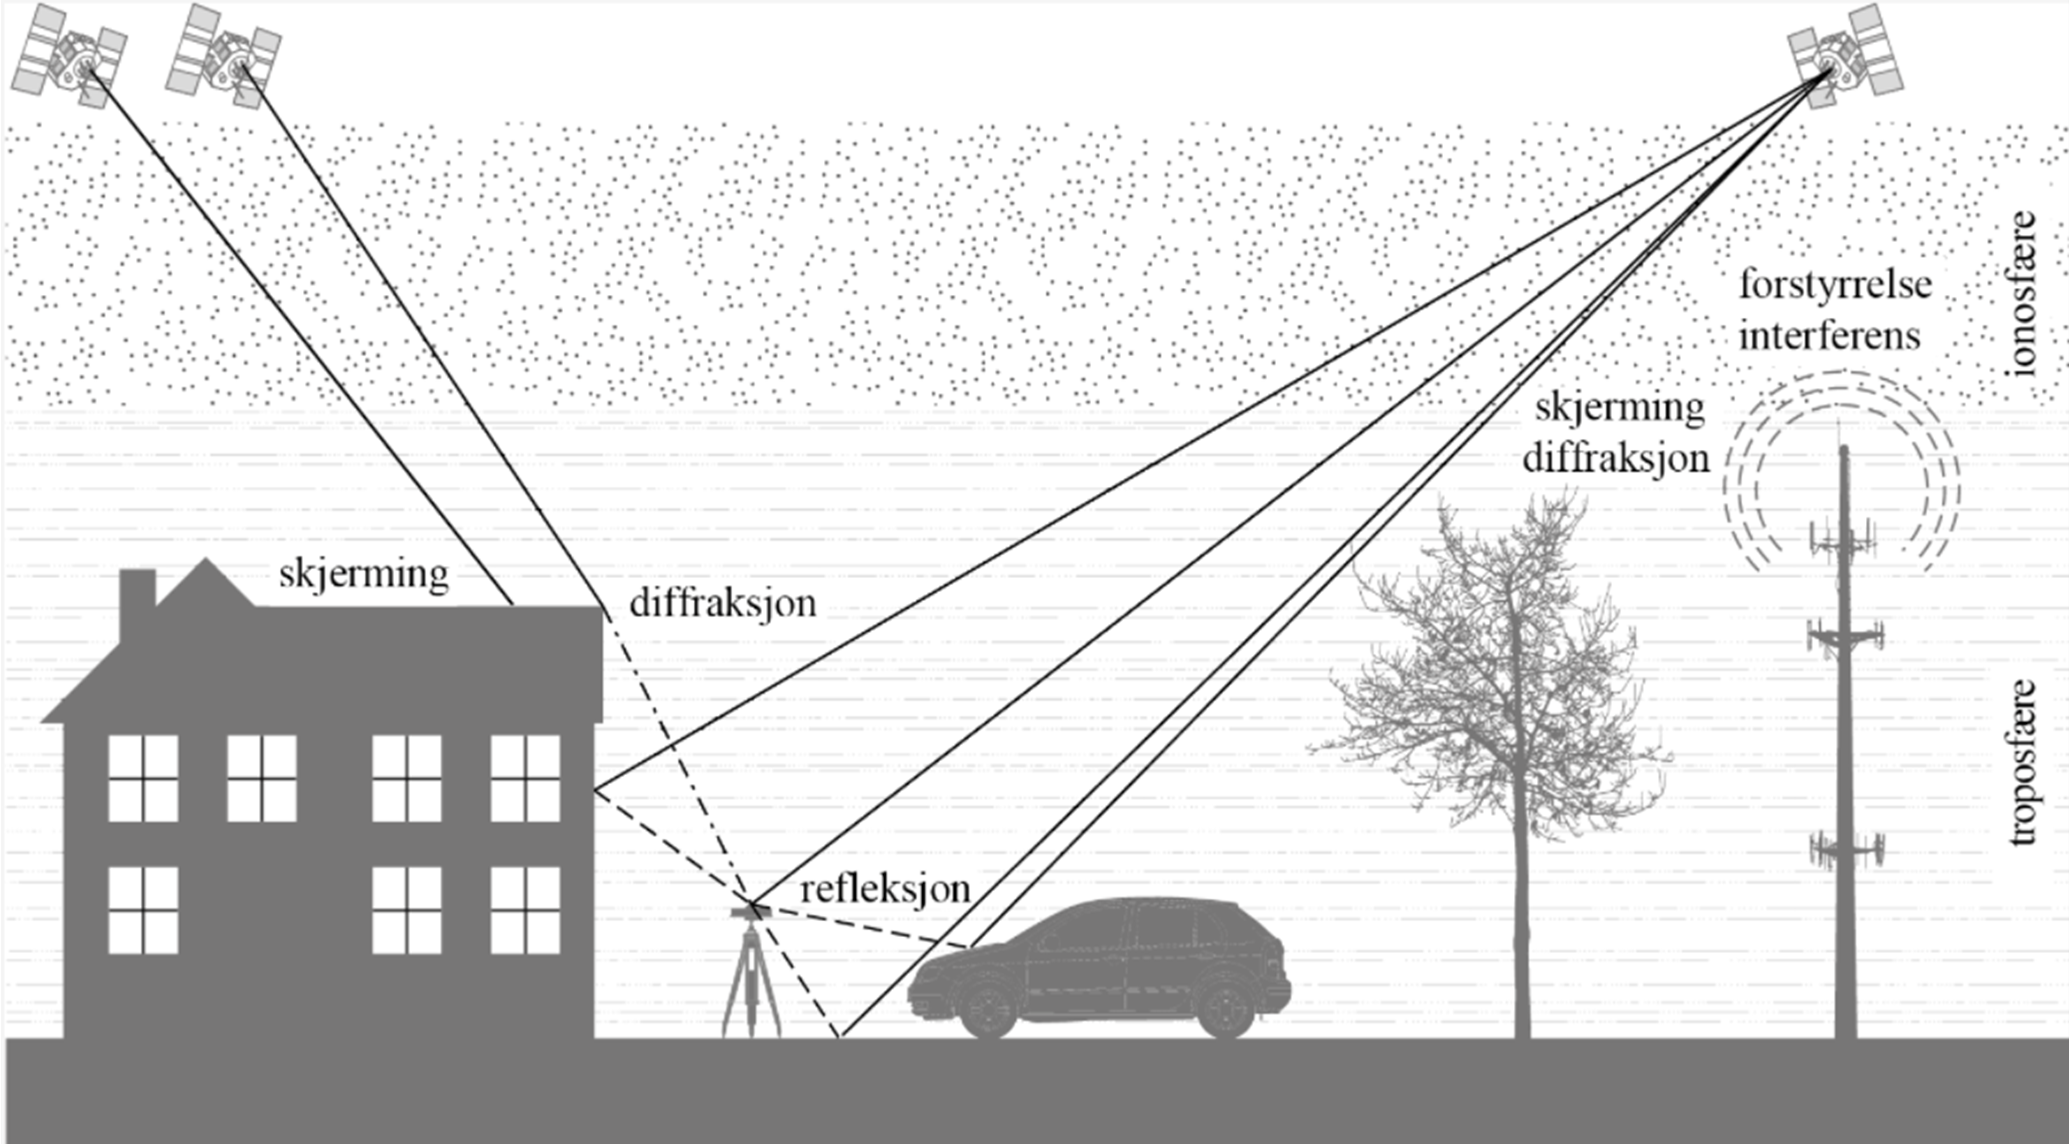
\includegraphics[width=1\columnwidth]{figures/gnss-feilkilder}
    \caption{GNSS-feilkilder.\parencite{NorskRomsenter}}
    \label{fig:gnss-feilkilder}
\end{figure}

GNSS utsettes for en rekke feilkilder som gjør at det er vanskelig å oppnå den teoretisk mulige nøyaktigheten. 
Figur \ref{fig:gnss-feilkilder} illustrerer de forskjellige feilkildene GNSS er utsatt for.

\begin{itemize}
\item Det kan oppstå feil i banedataen til satellittene. Dette kan komme av teknisk feil, eller at det er lenge siden banedataen er oppdatert. Dette vil føre til at GNSS-mottakeren beregner sin posisjon basert på feil posisjon på satellittene.
\item Signalene fra satellittene går i lysets hastighet, men de forsinkes noe gjennom atmosfæren, hvor blant annet luft bremser hastigheten. Hvis lokale forhold gjør at signalene forsinkes mer enn vanlig kan dette fremtvinge flere meter avvik i posisjon.
\item Hvis mottakeren ikke har klar sikt i alle himmelretninger, kan dette dekke for satellitter. Dette kan gjøre at posisjonen beregnes med færre satellitter enn ønskelig. Noe som fører til lavere nøyaktighet.
\item GNSS-signalene har svært lav effekt, og vil derfor lett kunne forstyrres av lokale signaler i nærheten av mottakeren som oppleves sterkere og som bruker omtrentlig lik frekvens som GNSS.
\item GNSS-signalene har en liten, men ikke neglisjerbar evne til å bøye seg rundt hindringer. Dette kan føre til at en mottaker som egentlig er skjult for en satellitt mottar signaler likevel. Disse signalene vil avvike fra den faktiske distansen til satellitten.
\item Signalene har lett for å reflektere fra overflater og gi falske forsinkede signaler til mottakeren. Dette er vanlig i urbane områder hvor det er mange blanke og flate overflater som kan reflektere signalene. Det kan også forekomme i naturen i nærheten av fjell og vann som har reflekterende egenskaper. \parencite{NorskRomsenter} 
\end{itemize}

I tillegg til disse feilkildene vil satellittenes posisjon i forhold til hverandre påvirke nøyaktigheten. 
Hvis en mottaker benytter satellitter som ligger svært tett eller på rekke, vil nøyaktigheten påvirkes negativt. 
Det er fordelaktig med satellitter med god spredning slik at vinklene mellom dem blir størst mulig. 
Dette gjør at krysningspunktene mellom radiene til hver satellitt blir minst mulig. \parencite{NorskRomsenter}